\documentclass{article}

% NeurIPS template, preprint mode. Put the official style file next to this file and, if your
% download has a different year (e.g. neurips_2026.sty), change the name below.
\usepackage[preprint]{neurips_2026}

\usepackage[utf8]{inputenc}
\usepackage[T1]{fontenc}
\usepackage{hyperref}
\usepackage{url}
\usepackage{booktabs}
\usepackage{amsfonts}
\usepackage{nicefrac}
\usepackage{microtype}
\usepackage{xcolor}
\usepackage{graphicx}
\usepackage{tikz}
\usetikzlibrary{arrows.meta,positioning}

\title{Reading Scanned and Photographed MCQ Answer Sheets \\ with a Template-Registration and Bubble-Darkness Pipeline}

% EDIT: your name, student number, e-mail
\author{%
  Rosheni Saraladevi Ramesh Babu \\
  School of Computer Science, University College Dublin \\
  Student number: 26100145 \\
  \texttt{rosheni.saraladevirameshba@ucdconnect.ie}
}

\begin{document}
\maketitle

\begin{abstract}
We build an automatic reader for scanned and photographed S3231 multiple-choice answer sheets
(120 questions with options A--E and an 8-digit student number). The system is a classical,
CPU-only pipeline: the page is registered to a canonical template with SIFT features and a RANSAC
homography (with a contour-based fallback), a bubble layout is learned from the registered
training pages, and each bubble is scored by pencil darkness measured in the red channel, where
the pink print is nearly invisible. A threshold rule with a blank option produces the answers, and
a local alignment of the student-number block improves digit reading. On 845 held-out test forms
from unseen students the system reaches 0.895 per-question accuracy, 0.909 student-number accuracy
and 0.173 exact-form accuracy, against 0.477 / 0.182 / 0.000 for a contour-warp baseline and
0.455 / 0.828 / 0.000 for plain argmax decoding. On a 90-form stress set the per-question accuracy
is 0.849, but student-number reading degrades to 0.256. An error analysis shows that failures are
concentrated: the worst 10\% of forms account for 56\% of all missed marks, mostly very faint
pencil on tinted paper. We discuss these limits, the cost of inference, and negative results.
\end{abstract}

\section{Introduction}
Optical mark recognition is a standard task, but exam sheets that students fill in by hand and
that are later captured with a phone camera, rather than a dedicated scanner, are harder than the
clean case: perspective, shadows, colour casts, curled paper and light pencil all change how a
bubble looks. The task here is to turn one image of an S3231 sheet into a JSON object with the
student number, the 120 answers (a letter or \texttt{null} for blank or ambiguous), and optional
header fields. The metrics are student-number accuracy, per-question accuracy, exact-form accuracy
(all 120 answers and the student number correct) and inference time, with a local CPU or GPU
implementation of at most 3\,GB of GPU memory.

We deliberately choose a classical pipeline. The sheet has a fixed printed layout, so the problem
is mostly geometric: if the page is registered precisely to a template, reading a bubble reduces to
measuring how dark it is. This gives a system that needs no learned weights, runs in well under a
second per form on a CPU, and whose failures can be inspected directly. Our contributions are
(i) a complete registration--layout--decoding pipeline with a documented evaluation protocol,
(ii) two baselines and four ablations, including negative results, and (iii) an error analysis that
separates registration failures from ink-contrast failures.

\section{Task and data}
\paragraph{Forms.} Each sheet has four groups of 30 questions with five options, a block of
8 digit columns for the student number, and header fields (name, module code, seat number, date).
Marks are pencil; the printed bubbles and text are pink or black.

\paragraph{Main dataset.} The main dataset has 2{,}094 labelled forms captured in three conditions:
flatbed scan, phone photo, and ``hard'' phone photo (strong perspective, shadows or cluttered
background). Labels are the 120 answers and the student number. We split by student, so that no
student appears in both parts, into 1{,}249 training and 845 test forms (test: 279 scan, 280 photo,
286 hard), and assert in code that the two parts share no student. About 12\% of test forms have no
valid 8-digit ground-truth student number; we keep them in the dataset and report student-number
accuracy both over all forms and over forms with a valid label.

\paragraph{Stress set.} A separate set of 90 forms (three held-out participants) is used only for
the final stress evaluation. Thresholds and all design choices were selected on the training part
of the main dataset. We note in Section~\ref{sec:honesty} one respect in which the stress set was
nevertheless seen during development.

\section{Method}
Figure~\ref{fig:pipeline} summarises the pipeline.

\begin{figure}[t]
\centering
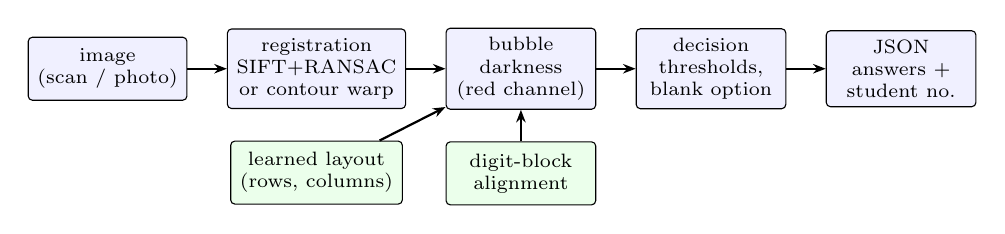
\begin{tikzpicture}[node distance=5mm, every node/.style={font=\scriptsize},
  box/.style={draw, rounded corners=1.5pt, minimum height=8mm, minimum width=19mm, align=center, fill=blue!6},
  arr/.style={-{Stealth[length=1.6mm]}, thick}]
  \node[box] (in) {image\\(scan / photo)};
  \node[box, right=of in] (reg) {registration\\SIFT+RANSAC\\or contour warp};
  \node[box, right=of reg] (bub) {bubble\\darkness\\(red channel)};
  \node[box, right=of bub] (dec) {decision\\thresholds,\\blank option};
  \node[box, right=of dec] (out) {JSON\\answers +\\student no.};
  \draw[arr] (in)--(reg); \draw[arr] (reg)--(bub); \draw[arr] (bub)--(dec); \draw[arr] (dec)--(out);
  \node[box, below=4mm of reg, fill=green!8] (lay) {learned layout\\(rows, columns)};
  \node[box, below=4mm of bub, fill=green!8] (al) {digit-block\\alignment};
  \draw[arr] (lay)--(bub); \draw[arr] (al)--(bub);
\end{tikzpicture}
\caption{Pipeline. The layout is learned once from registered training pages; the digit-block
alignment is estimated per form.}
\label{fig:pipeline}
\end{figure}

\subsection{Registration}
Every form is registered to a canonical template page, the median of well-registered training
pages. We detect SIFT keypoints~\citep{lowe2004} on the input and on the template, match them with
a ratio test, and estimate a homography with RANSAC~\citep{fischler1981,hartley2004} using
OpenCV~\citep{bradski2000}. If this fails, or if the registered page is a poor match, we fall
back to a contour-based page detector with a perspective warp. A match score,
the cosine similarity between down-sampled print maps (green channel) of the registered page and
the template, triggers up to three retries with different SIFT settings and the contour fallback;
the best-scoring result is kept. On the test set 780 forms use the default SIFT setting, 42 a
retry setting, 20 the contour warp and 3 the last-resort fallback.

\subsection{Layout}
After registration all sheets share one coordinate system. We learn the layout from the median of
registered training pages. Timing marks along the right edge give the row positions, and peak
finding on column profiles gives the bubble columns: four answer groups of five columns, eight
digit columns, and a nine-row digit grid. The learned layout is stored in a small JSON file
together with the bubble half-size. Overlaying predictions on pages and auditing the ink at labelled
bubbles revealed an early off-by-one in the learned rows (the digit grid had absorbed the first
answer row); fixing it raised per-question accuracy on test forms from 0.560, no better than reporting every
question as blank, to 0.895.

\subsection{Bubble darkness}
The pink printing is bright in the red channel, so pencil is the dominant dark signal there. We
divide the red channel by a smoothed local background (grey dilation followed by Gaussian blur)
to flatten shadows, define ink $=1-r/\mathrm{bg}$ clipped to $[0,1]$, and score each bubble as the
mean ink inside a box around its centre, computed with an integral image.

\subsection{Decision rule}
For a group of options with scores $s_1\ge s_2\ge\dots$ the answer is the arg-max option if
$s_1\ge \tau_{abs}$ and $s_2\le\tau_{rel}\,s_1$; otherwise it is \texttt{null}. Answers and
student-number digits have separate thresholds, tuned on the training part by grid search over
$\tau_{abs}\in[0.02,0.39]$ and $\tau_{rel}\in\{0.4,\dots,0.9\}$, with and without subtracting the
form's median bubble darkness. The selected values are $\tau_{abs}=0.02,\ \tau_{rel}=0.8$ for answers
and $0.03,\ 0.9$ for digits, without median subtraction. A student number is returned only if all
eight digit columns are decided, otherwise \texttt{null}.

\subsection{Digit-block alignment}
Registration can leave a block a few pixels off. For the student-number block only, we search
shifts of up to $\pm10$\,px horizontally and $\pm14$\,px vertically and keep the shift that
maximises the mean over columns of (darkest bubble $-$ median bubble), with a small penalty on the
shift size. This exploits the fact that each digit column holds exactly one mark.

\section{Experimental protocol}
All thresholds are tuned on the training part only. Baselines use the same bubble reader with one
component removed (the contour baseline reuses our tuned thresholds): \emph{contour warp only} replaces registration by the
contour page detector; \emph{plain argmax} always returns the darkest option, with no blank
option. We report student-number accuracy (exact 8-digit match; a form with an invalid label counts
as correct only if the prediction is \texttt{null}), per-question accuracy over all $120$ answers
including blanks, and exact-form accuracy. Inference time is the per-form processing time inside the
batch pipeline, plus the end-to-end time of the \texttt{predict.py} command-line tool on CPU.

\section{Results}
\begin{table}[t]
\centering\small
\caption{Test-set results (845 forms) and stress-set results (90 forms). Time is per form inside
the batch pipeline on CPU.}
\label{tab:main}
\begin{tabular}{lrrrr}
\toprule
Method & Student no. & Per-question & Exact form & Time (s) \\
\midrule
Ours (test)                     & \textbf{0.909} & \textbf{0.895} & \textbf{0.173} & 0.087 \\
Contour warp only (test)        & 0.182 & 0.477 & 0.000 & 0.193 \\
Plain argmax, no blank (test)   & 0.828 & 0.455 & 0.000 & 0.087 \\
\midrule
Ours (stress)                   & 0.256 & 0.849 & 0.044 & 0.094 \\
\bottomrule
\end{tabular}
\end{table}

Table~\ref{tab:main} and Figure~\ref{fig:results} give the main results. Registration is the most
important component: the contour warp alone loses 42 points of per-question accuracy and 73
points of student-number accuracy, since a page-contour warp is a coarser registration than feature
matching and leaves bubbles off-centre. The blank option is the second most important: plain argmax
always reports a letter, so it reads the 52\% of questions that are blank as answers, which cuts
per-question accuracy to 0.455; its student-number accuracy (0.828) is also lower than ours partly
because it can never return \texttt{null} for a form without a valid label. Exact-form accuracy is
low for every method, since a single wrong answer out of 120 makes a form incorrect. With independent
errors, 0.895 per question would give an exact-form rate close to zero; the observed 0.173 shows that
errors are clustered in a minority of forms (Section~\ref{sec:err}).

\begin{figure}[t]
\centering
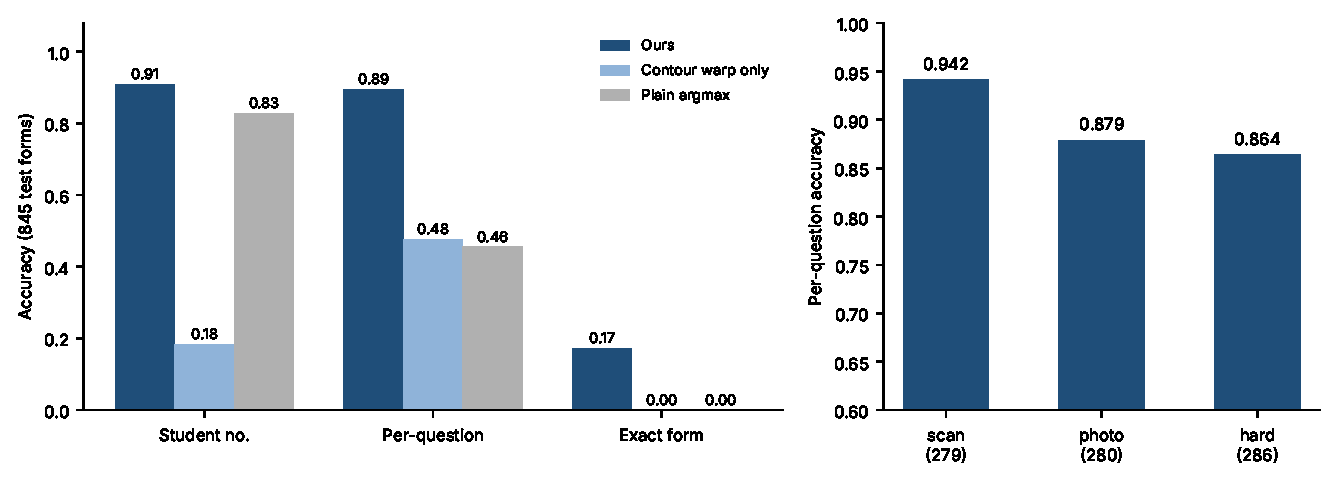
\includegraphics[width=0.93\linewidth]{fig_results.pdf}
\caption{Left: test accuracy of our system and the two baselines. Right: per-question accuracy
by capture condition (scan 279 forms, photo 280, hard 286).}
\label{fig:results}
\end{figure}

\paragraph{By capture condition and registration method.} Per-question accuracy is 0.942 on scans,
0.879 on photos and 0.864 on hard photos. By registration method it is 0.907 for the default
SIFT setting ($n{=}780$), 0.906 for the retry setting (42), 0.503 for the contour fallback (20) and
0.225 for the last-resort fallback (3). Registration failures are rare (23 of 845 forms) but costly.

\paragraph{Ablations.} Table~\ref{tab:abl} lists the changes we tried beyond the baseline reader.
Aligning the digit block is the only one that helped clearly (student-number accuracy on forms with
a valid label rose from 0.891 to 0.914 on test). The same alignment applied to each answer group
\emph{hurt}: per-question accuracy fell from 0.895 to 0.871 and false letters on blank questions
rose from 753 to 2{,}624 for option A. The alignment criterion rewards dark structure, and the left
edge of each answer group contains printed structure that is not a mark; digit columns, in contrast,
contain exactly one mark. A per-form normalisation of bubble scores (median and 95th percentile)
lowered test accuracy to 0.866. A per-form Otsu threshold~\citep{otsu1979} gave a small gain
(0.898 vs.\ 0.895); we did not adopt it because the difference is within what one would expect from
noise on this split and it complicates the decision rule.

\begin{table}[t]
\centering\small
\caption{Ablations on the test set (per-question accuracy unless stated).}
\label{tab:abl}
\begin{tabular}{lrl}
\toprule
Change & Result & Adopted \\
\midrule
Digit-block alignment & student no. 0.891 $\to$ 0.914 (valid labels) & yes \\
Answer-group alignment & 0.895 $\to$ 0.871 & no \\
Per-form normalisation (median, 95th pct.) & 0.895 $\to$ 0.866 & no \\
Per-form Otsu threshold & 0.895 $\to$ 0.898 & no \\
Median subtraction in the threshold rule & train answers 0.862 vs.\ 0.884 (without) & no \\
\bottomrule
\end{tabular}
\end{table}

\section{Error analysis}\label{sec:err}
Figure~\ref{fig:conf} shows the per-question confusion matrix on test forms. Of the 49{,}167
marked questions, 40{,}300 (82.0\%) are read correctly, 7{,}737 (15.7\%) are read as blank and
1{,}130 (2.3\%) as a wrong letter; of the 52{,}233 blank questions, 1{,}818 (3.5\%) are read
as a letter. Almost all errors are therefore missed marks, not confusions between letters.

\begin{figure}[t]
\centering
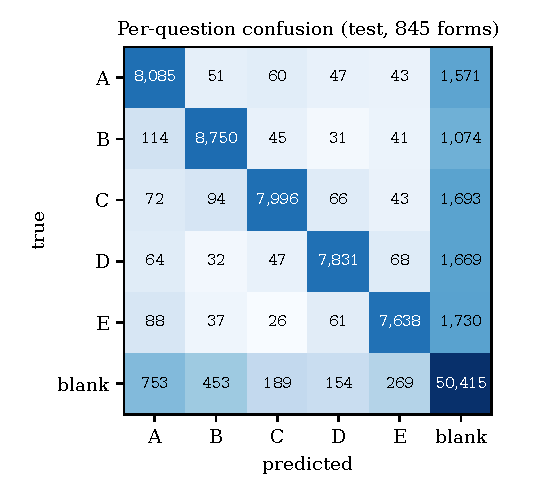
\includegraphics[width=0.55\linewidth]{fig_confusion.pdf}
\caption{Per-question confusion matrix on the 845 test forms (colour is log counts).}
\label{fig:conf}
\end{figure}

\paragraph{Errors are concentrated.} A typical form is almost error-free: the median form has one
missed mark and one false mark. The mean is 9.2 missed marks per form because a minority of
forms fail almost completely: the worst 10\% of forms contain 56\% of all misses, and the ten worst
miss between 80 and 103 of 111--118 marks. In the overlays of the four we inspected the pages are
well registered but the marks are very faint. On the ten worst forms, the mean ink at marked
bubbles is only 0.01--0.05 above the mean ink at blank bubbles (e.g.\ 0.204 vs.\ 0.166 for one scan),
and the blank-bubble level is itself high (0.11--0.20), which we attribute to the paper tint and
colour casts visible in the images. A rank statistic comparing marked
to blank bubbles on those ten forms (AUC) ranges from 0.54 to 0.90, so some forms could be read with
a form-specific threshold, while others (AUC 0.54--0.58) carry almost no usable contrast in the
red channel. This is a limit of the sensing channel, not only of the threshold.

\paragraph{Student number.} On test forms with a valid label, 91.4\% of student numbers are exact,
with 95--96\% per-column accuracy and about 2--3\% blank reads per column. The 12\% of forms without a
valid label cannot be scored against an 8-digit ground truth. On the stress set, only 21\% of
valid student numbers are exact, with 36--57\% per-column accuracy and 7--15\% blank reads: the
student-number block sits in the top of the page, where registration of tilted phone photos is
least precise and where we found offsets of one row in individual forms.

\IfFileExists{fig_examples.pdf}{%
\begin{figure}[t]
\centering
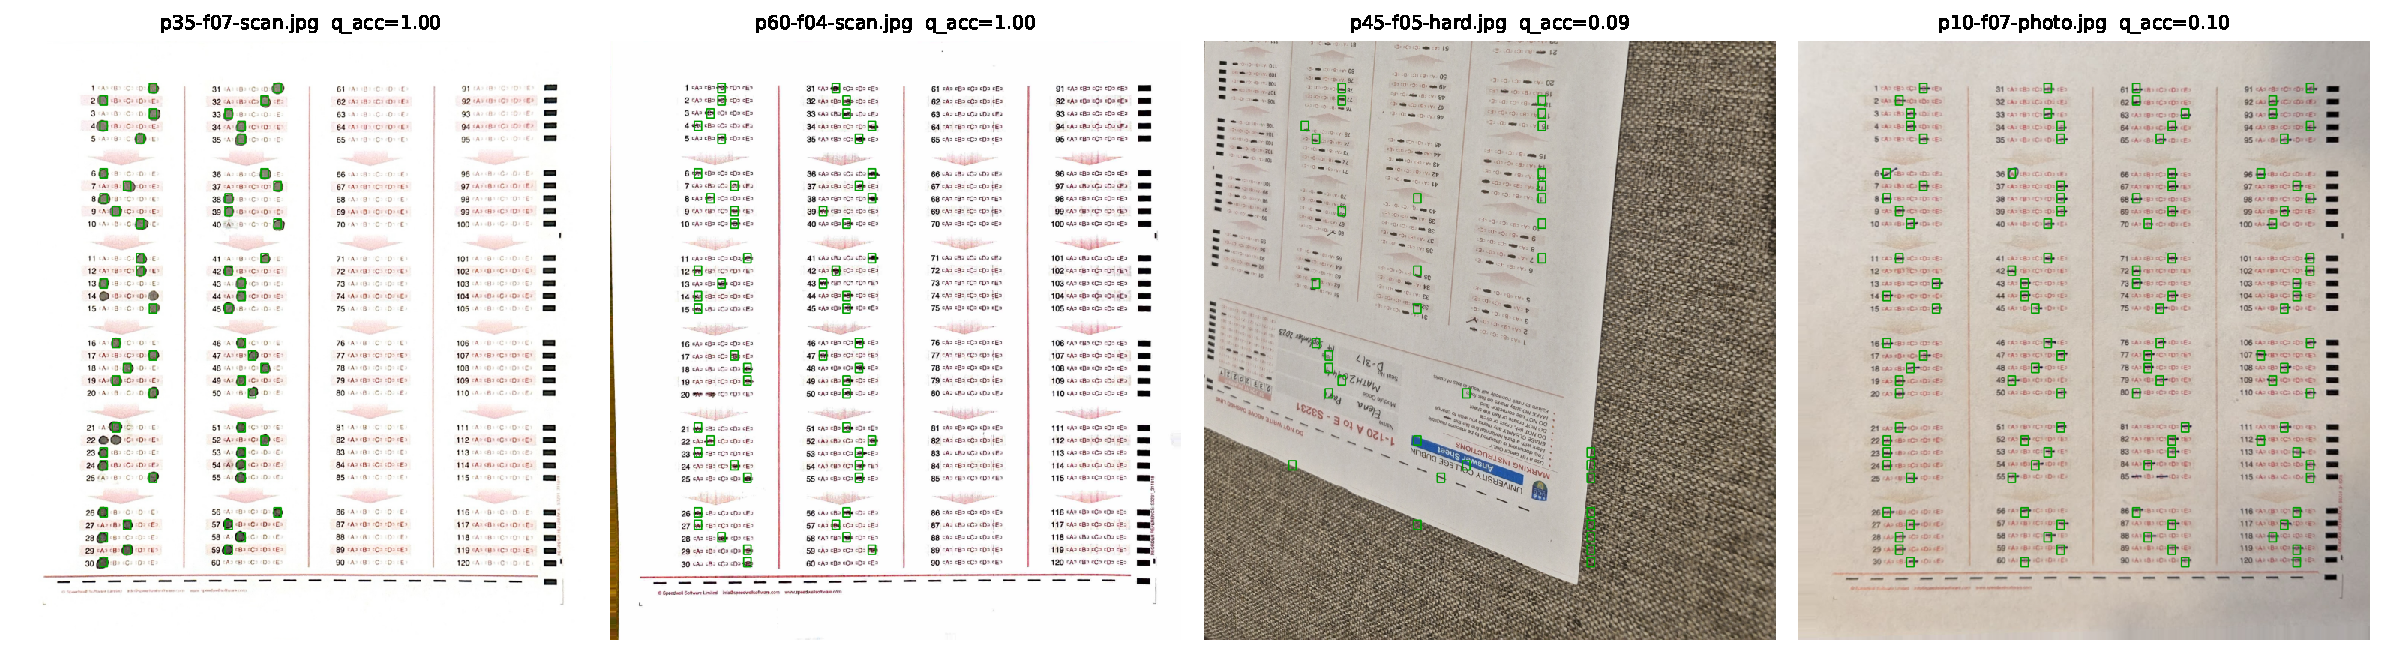
\includegraphics[width=\linewidth]{fig_examples.pdf}
\caption{Predicted answers (green boxes) on registered test pages, answer area only. The two left
examples are the best cases; the two right examples are the worst, with very faint pencil
or strong perspective.}
\label{fig:examples}
\end{figure}}{}

\section{Robustness, limitations and cost}
\paragraph{Robustness.} \texttt{predict.py} always writes valid JSON with the six required fields.
On an unreadable file, a missing file or any internal error it writes \texttt{null} for every field
and exits normally. We checked this on a corrupt file and a non-existent path, and ran the tool
end to end in a fresh virtual environment built from \texttt{requirements.txt}.

\paragraph{Limitations.} (i) The header fields (name, module code, seat number, date) are not
recognised and are returned as \texttt{null}; this would need handwriting OCR. (ii) Faint pencil on
tinted paper is the main failure mode and caused most of the missed marks. (iii) Erasures and
double marks are not modelled beyond returning \texttt{null}. (iv) The student-number grid in our
layout has nine digit rows and none of the ground-truth student numbers contains a 9. (v) Stress
student-number accuracy is poor, so for photos taken under conditions unlike the training photos the
student number should not be trusted without review. (vi) Exact-form accuracy is low
(0.173), so the system is better suited to assisting a marker than to unsupervised marking.

\paragraph{Cost.} The system uses no GPU and no learned neural weights. Its parameters are a
learned layout, a canonical template image and five thresholds, stored in three small files. Per-form
processing time is about 0.09\,s in the batch pipeline and 1.4\,s for the command-line tool,
including interpreter and OpenCV start-up and loading the template, on a laptop CPU.
The extra registration retries cost time but did not give a measurable aggregate gain in our
runs; they remain in the system to handle the few forms where the default SIFT setting fails.

\section{Honest account of the evaluation}\label{sec:honesty}
Thresholds were tuned on the training part only and all numbers above are from forms not used
for tuning. Two caveats apply. First, the stress forms were inspected while diagnosing the low
student-number accuracy; this motivated the digit-block alignment, which we then validated on the
test split, and we made no further changes based on stress forms, but the stress result is not
fully blind to that design decision. Second, the ground-truth student numbers are invalid for
about 12\% of forms, which limits how precisely student-number accuracy can be measured.

\section{Conclusion}
A template-registration and bubble-darkness pipeline reads most answers on unseen students'
scans and photos using only a CPU. Its errors are dominated by missed marks on a minority of
low-contrast forms and by registration of the student-number block on tilted photos. Natural next
steps are a per-form contrast model trained on the labelled bubbles, a registration refinement
using the printed timing marks of each form, and handwriting recognition for the header fields.

\section*{Contribution and use of AI assistance}
% EDIT so that this matches exactly what you did, and follow the course policy on AI use.
The author designed and ran all experiments in the evaluation notebook, chose the evaluation
protocol and wrote this report. An AI coding assistant (Claude) was used to help write and debug
parts of the code and to suggest diagnostics and ablations; the author ran the code, inspected the
outputs and made the decisions on what to keep. The dataset was provided by the course.

\small
\begin{thebibliography}{9}
\bibitem[Bradski(2000)]{bradski2000} G.~Bradski. The OpenCV library. \emph{Dr.\ Dobb's Journal of Software Tools}, 2000.
\bibitem[Fischler and Bolles(1981)]{fischler1981} M.~A. Fischler and R.~C. Bolles. Random sample consensus: a paradigm for model fitting with applications to image analysis and automated cartography. \emph{Communications of the ACM}, 24(6):381--395, 1981.
\bibitem[Hartley and Zisserman(2004)]{hartley2004} R.~Hartley and A.~Zisserman. \emph{Multiple View Geometry in Computer Vision}. Cambridge University Press, 2nd edition, 2004.
\bibitem[Lowe(2004)]{lowe2004} D.~G. Lowe. Distinctive image features from scale-invariant keypoints. \emph{International Journal of Computer Vision}, 60(2):91--110, 2004.
\bibitem[Otsu(1979)]{otsu1979} N.~Otsu. A threshold selection method from gray-level histograms. \emph{IEEE Transactions on Systems, Man, and Cybernetics}, 9(1):62--66, 1979.
\end{thebibliography}

\end{document}